\documentclass[12pt,a4paper]{article}

\usepackage{amsfonts}
\usepackage[centertags]{amsmath}
\usepackage{amsthm}
\usepackage{amssymb}

\usepackage[utf8]{inputenc}
\usepackage[french]{babel}

\usepackage{graphicx}

\leftmargin=0pt \topmargin=0pt \headheight=0in \headsep=0in \oddsidemargin=0pt \textwidth=6.5in
\textheight=8.5in


% Schriftabk¸rzungen

\newcommand{\eps}{\varepsilon}
\renewcommand{\phi}{\varphi}
\newcommand{\Sl}{\ell}    % schÀÜnes l
\newcommand{\ve}{\varepsilon}  %Epsilon

\newcommand{\BA}{{\mathbb{A}}}
\newcommand{\BB}{{\mathbb{B}}}
\newcommand{\BC}{{\mathbb{C}}}
\newcommand{\BD}{{\mathbb{D}}}
\newcommand{\BE}{{\mathbb{E}}}
\newcommand{\BF}{{\mathbb{F}}}
\newcommand{\BG}{{\mathbb{G}}}
\newcommand{\BH}{{\mathbb{H}}}
\newcommand{\BI}{{\mathbb{I}}}
\newcommand{\BJ}{{\mathbb{J}}}
\newcommand{\BK}{{\mathbb{K}}}
\newcommand{\BL}{{\mathbb{L}}}
\newcommand{\BM}{{\mathbb{M}}}
\newcommand{\BN}{{\mathbb{N}}}
\newcommand{\BO}{{\mathbb{O}}}
\newcommand{\BP}{{\mathbb{P}}}
\newcommand{\BQ}{{\mathbb{Q}}}
\newcommand{\BR}{{\mathbb{R}}}
\newcommand{\BS}{{\mathbb{S}}}
\newcommand{\BT}{{\mathbb{T}}}
\newcommand{\BU}{{\mathbb{U}}}
\newcommand{\BV}{{\mathbb{V}}}
\newcommand{\BW}{{\mathbb{W}}}
\newcommand{\BX}{{\mathbb{X}}}
\newcommand{\BY}{{\mathbb{Y}}}
\newcommand{\BZ}{{\mathbb{Z}}}

\newcommand{\Fa}{{\mathfrak{a}}}
\newcommand{\Fb}{{\mathfrak{b}}}
\newcommand{\Fc}{{\mathfrak{c}}}
\newcommand{\Fd}{{\mathfrak{d}}}
\newcommand{\Fe}{{\mathfrak{e}}}
\newcommand{\Ff}{{\mathfrak{f}}}
\newcommand{\Fg}{{\mathfrak{g}}}
\newcommand{\Fh}{{\mathfrak{h}}}
\newcommand{\Fi}{{\mathfrak{i}}}
\newcommand{\Fj}{{\mathfrak{j}}}
\newcommand{\Fk}{{\mathfrak{k}}}
\newcommand{\Fl}{{\mathfrak{l}}}
\newcommand{\Fm}{{\mathfrak{m}}}
\newcommand{\Fn}{{\mathfrak{n}}}
\newcommand{\Fo}{{\mathfrak{o}}}
\newcommand{\Fp}{{\mathfrak{p}}}
\newcommand{\Fq}{{\mathfrak{q}}}
\newcommand{\Fr}{{\mathfrak{r}}}
\newcommand{\Fs}{{\mathfrak{s}}}
\newcommand{\Ft}{{\mathfrak{t}}}
\newcommand{\Fu}{{\mathfrak{u}}}
\newcommand{\Fv}{{\mathfrak{v}}}
\newcommand{\Fw}{{\mathfrak{w}}}
\newcommand{\Fx}{{\mathfrak{x}}}
\newcommand{\Fy}{{\mathfrak{y}}}
\newcommand{\Fz}{{\mathfrak{z}}}

\newcommand{\FA}{{\mathfrak{A}}}
\newcommand{\FB}{{\mathfrak{B}}}
\newcommand{\FC}{{\mathfrak{C}}}
\newcommand{\FD}{{\mathfrak{D}}}
\newcommand{\FE}{{\mathfrak{E}}}
\newcommand{\FF}{{\mathfrak{F}}}
\newcommand{\FG}{{\mathfrak{G}}}
\newcommand{\FH}{{\mathfrak{H}}}
\newcommand{\FI}{{\mathfrak{I}}}
\newcommand{\FJ}{{\mathfrak{J}}}
\newcommand{\FK}{{\mathfrak{K}}}
\newcommand{\FL}{{\mathfrak{L}}}
\newcommand{\FM}{{\mathfrak{M}}}
\newcommand{\FN}{{\mathfrak{N}}}
\newcommand{\FO}{{\mathfrak{O}}}
\newcommand{\FP}{{\mathfrak{P}}}
\newcommand{\FQ}{{\mathfrak{Q}}}
\newcommand{\FR}{{\mathfrak{R}}}
\newcommand{\FS}{{\mathfrak{S}}}
\newcommand{\FT}{{\mathfrak{T}}}
\newcommand{\FU}{{\mathfrak{U}}}
\newcommand{\FV}{{\mathfrak{V}}}
\newcommand{\FW}{{\mathfrak{W}}}
\newcommand{\FX}{{\mathfrak{X}}}
\newcommand{\FY}{{\mathfrak{Y}}}
\newcommand{\FZ}{{\mathfrak{Z}}}

\newcommand{\CA}{{\cal A}}
\newcommand{\CB}{{\cal B}}
\newcommand{\CC}{{\cal C}}
\newcommand{\CD}{{\cal D}}
\newcommand{\CE}{{\cal E}}
\newcommand{\CF}{{\cal F}}
\newcommand{\CG}{{\cal G}}
\newcommand{\CH}{{\cal H}}
\newcommand{\CI}{{\cal I}}
\newcommand{\CJ}{{\cal J}}
\newcommand{\CK}{{\cal K}}
\newcommand{\CL}{{\cal L}}
\newcommand{\CM}{{\cal M}}
\newcommand{\CN}{{\cal N}}
\newcommand{\CO}{{\cal O}}
\newcommand{\CP}{{\cal P}}
\newcommand{\CQ}{{\cal Q}}
\newcommand{\CR}{{\cal R}}
\newcommand{\CS}{{\cal S}}
\newcommand{\CT}{{\cal T}}
\newcommand{\CU}{{\cal U}}
\newcommand{\CV}{{\cal V}}
\newcommand{\CW}{{\cal W}}
\newcommand{\CX}{{\cal X}}
\newcommand{\CY}{{\cal Y}}
\newcommand{\CZ}{{\cal Z}}

% Theorem Stil

\theoremstyle{plain}
\newtheorem{lem}{Lemma}
\newtheorem{Satz}[lem]{Satz}

\theoremstyle{definition}
\newtheorem{defn}{Definition}[section]

\theoremstyle{remark}
\newtheorem{bem}{Bemerkung}    %[section]



\newcommand{\card}{\mathop{\rm card}\nolimits}
\newcommand{\Sets}{((Sets))}
\newcommand{\id}{{\rm id}}
\newcommand{\supp}{\mathop{\rm Supp}\nolimits}

\newcommand{\ord}{\mathop{\rm ord}\nolimits}
\renewcommand{\mod}{\mathop{\rm mod}\nolimits}
\newcommand{\sign}{\mathop{\rm sign}\nolimits}
\newcommand{\ggT}{\mathop{\rm ggT}\nolimits}
\newcommand{\kgV}{\mathop{\rm kgV}\nolimits}
\renewcommand{\div}{\, | \,}
\newcommand{\notdiv}{\mathopen{\mathchoice
             {\not{|}\,}
             {\not{|}\,}
             {\!\not{\:|}}
             {\not{|}}
             }}

\newcommand{\im}{\mathop{{\rm Im}}\nolimits}
\newcommand{\coim}{\mathop{{\rm coim}}\nolimits}
\newcommand{\coker}{\mathop{\rm Coker}\nolimits}
\renewcommand{\ker}{\mathop{\rm Ker}\nolimits}

\newcommand{\pRang}{\mathop{p{\rm -Rang}}\nolimits}
\newcommand{\End}{\mathop{\rm End}\nolimits}
\newcommand{\Hom}{\mathop{\rm Hom}\nolimits}
\newcommand{\Isom}{\mathop{\rm Isom}\nolimits}
\newcommand{\Tor}{\mathop{\rm Tor}\nolimits}
\newcommand{\Aut}{\mathop{\rm Aut}\nolimits}

\newcommand{\adj}{\mathop{\rm adj}\nolimits}

\newcommand{\Norm}{\mathop{\rm Norm}\nolimits}
\newcommand{\Gal}{\mathop{\rm Gal}\nolimits}
\newcommand{\Frob}{{\rm Frob}}

\newcommand{\disc}{\mathop{\rm disc}\nolimits}

\renewcommand{\Re}{\mathop{\rm Re}\nolimits}
\renewcommand{\Im}{\mathop{\rm Im}\nolimits}

\newcommand{\Log}{\mathop{\rm Log}\nolimits}
\newcommand{\Res}{\mathop{\rm Res}\nolimits}
\newcommand{\Bild}{\mathop{\rm Bild}\nolimits}

\renewcommand{\binom}[2]{\left({#1}\atop{#2}\right)}
\newcommand{\eck}[1]{\langle #1 \rangle}
\newcommand{\wi}{\hspace{1pt} < \hspace{-6pt} ) \hspace{2pt}}


\begin{document}

\pagestyle{empty}

\begin{center}
{\huge Lösungen zur Vorrundenprüfung 2011} \\
\end{center}
\vspace{8mm}

Zuerst einige Bemerkungen zum Punkteschema. Eine vollständige und korrekte Lösung einer Aufgabe ist jeweils 7 Punkte wert. Für Komplette Lösungen mit kleineren Fehlern oder Ungenauigkeiten, die aber keinen wesentlichen Einfluss auf die Richtigkeit der dargestellten Lösung haben, geben wir 6 Punkte. Bei unvollständigen Lösungen wird der Fortschritt und der Erkenntnissgewinn bewertet (Teilpunkte). Oft gibt es mehrere Lösungen für ein Problem. Versucht jemand zum Beispiel eine Aufgabe auf zwei verschiedenen Wegen zu lösen, erreicht auf dem ersten Weg 3 Punkte, auf dem zweiten 2 Punkte, dann wird seine Punktzahl nicht 5, sondern 3 sein. Punkte, die auf verschiedenen Wegen erreicht werden, sind also \emph{nicht} kumulierbar. Die unten angegebenen Bewertungsschemata sind nur Orientierungshilfe. Gibt jemand eine alternative Lösung, dann werden wir versuchen, die Punktzahl entsprechend zu wählen, dass für gleiche Leistung gleich viele Punkte verteilt werden. Die Schemata sind stets wie folgt zu interpretieren:\\
Kommt jemand in seiner Lösung bis und mit hierhin, dann gibt das soviele Punkte.\\ 
Ausnahmen von dieser Regel sind jeweils ausdrücklich deklariert.

\vspace{8mm}

\begin{enumerate}

\item[\textbf{1.}] 

\textbf{Erste Lösung}:\\
Es gilt $\angle MAB=90^\circ$ und somit ist der Kreis durch die Punkte $A, B, L$ und $M$ gerade der Thaleskreis über $MB$. Dann folgt aber sofort $\angle MLB=90^\circ$.
Analog erhält man $\angle NLC=90^\circ$. $M$ und $N$ liegen also beide auf der Senkrechten zu $BC$ durch $L$ und damit ist die Aussage bewiesen. \\

\begin{figure}[h]
\begin{center}
\includegraphics[width=13cm]{aufgabe1.pdf}
\caption{Aufgabe 1 - Skizze zur ersten Lösung}
\end{center}
\end{figure}

\textbf{Zweite Lösung}:\\
Sei $\angle ACB=\gamma$. Wir wählen unsere Skizze so, dass $L, M$ und $N$ nicht auf einer Geraden liegen (d.h. wir müssen unsere Skizze etwas ungenau zeichnen). Sei $M'$ der Schnittpunkt der Geraden $LN$ und $AC$. Wir sind fertig, wenn wir zeigen können, dass $M=M'$ gilt.\\
Wegen der Innenwinkelsumme im Dreieck ABC gilt: $\angle ABC=90^\circ-\gamma$. $MBLA$ ist ein Sehnenviereck, also gilt nach dem Peripheriewinkelsatz: $\angle AML=\angle ABL=90^\circ-\gamma$.\\
$ANLC$ ist ein Sehnenviereck, also ergänzen sich gegenüberliegende Winkel zu $180^\circ$ und somit gilt: $\angle ANL=180^\circ-\gamma$. Wegen dem Aussenwinkelsatz beim Dreieck $AM'N$ gilt $\angle ANL=\angle M'AN+\angle AM'N$ und somit $\angle AM'N=90^\circ-\gamma$.\\
Nun ist aber $\angle AML=\angle AM'L$, also sind die Geraden $M'L$ und $ML$ parallel. Die beiden Geraden enthalten aber beide $L$ als gemeinsamen Punkt, also sind sie sogar identisch und es folgt $M=M'$, womit wir fertig sind.\\

\begin{figure}[h]
\begin{center}
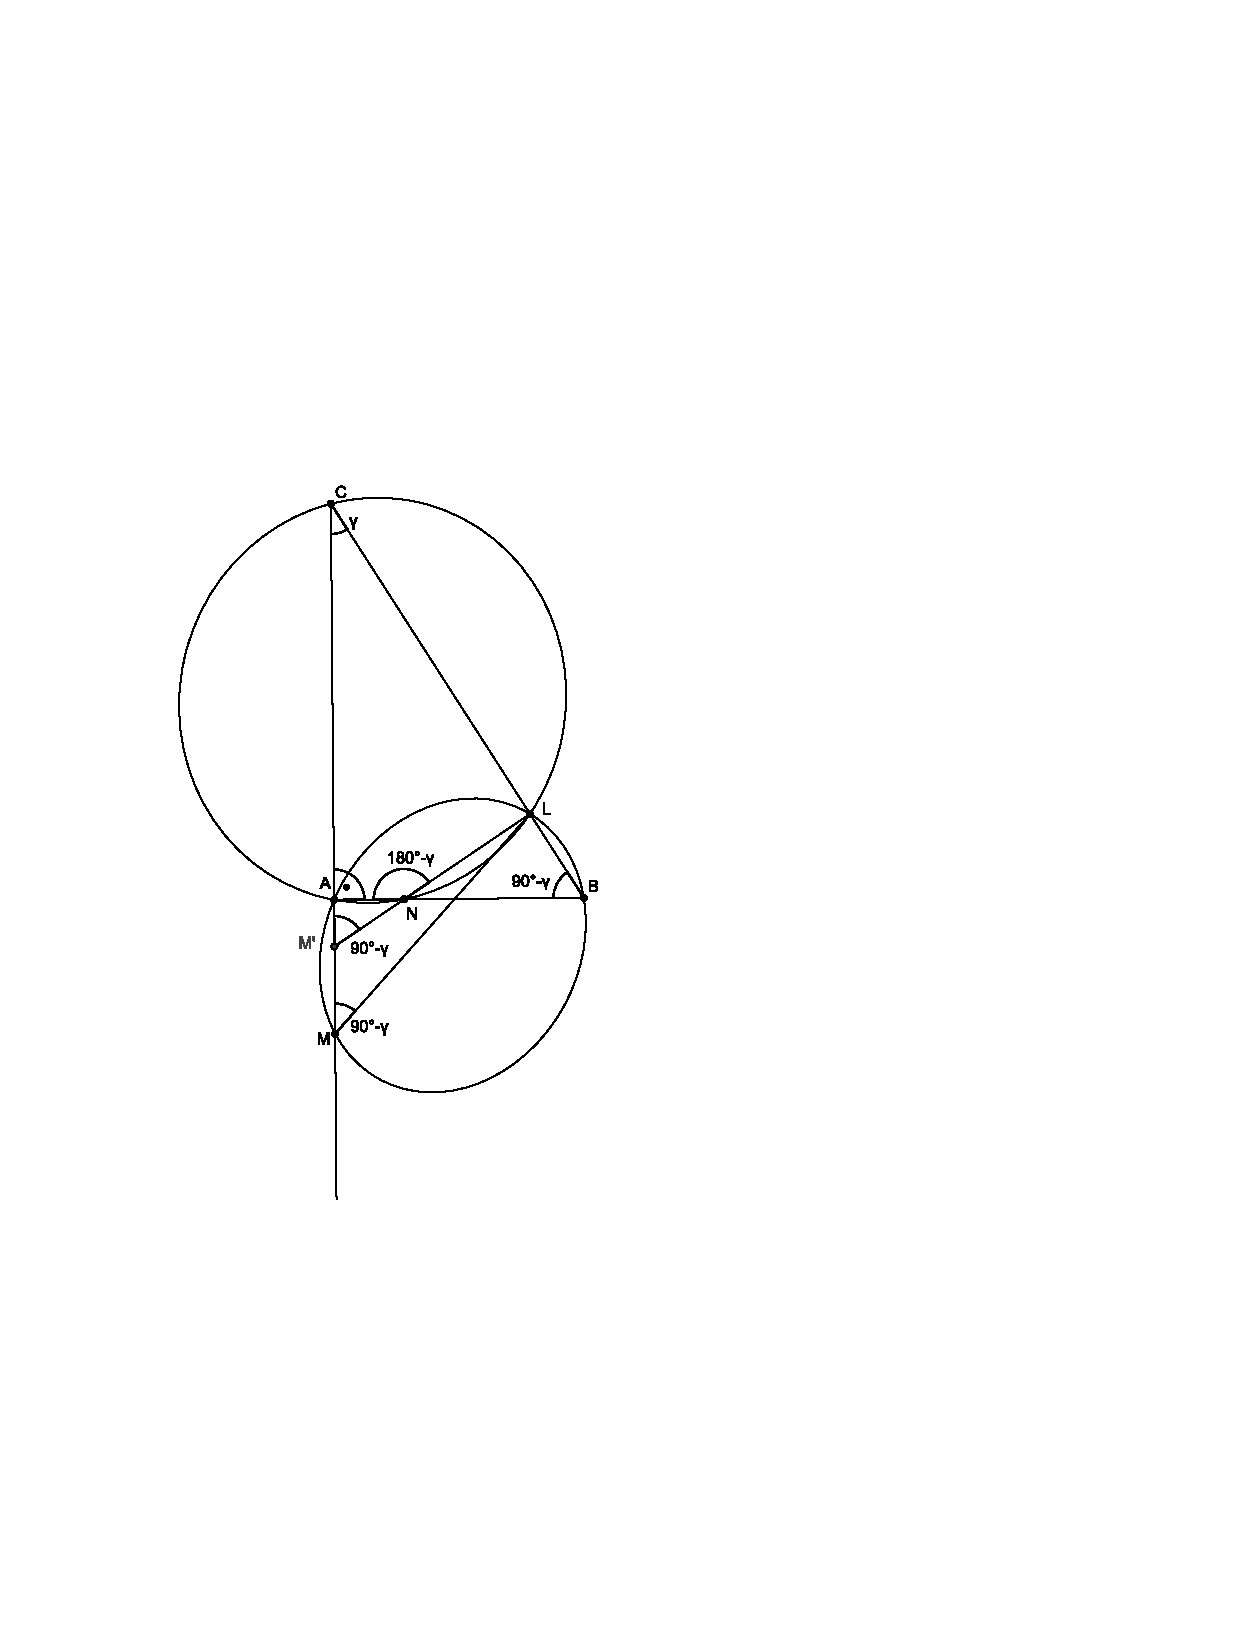
\includegraphics[width=8cm]{aufgabe1b.pdf}
\caption{Aufgabe 1 - Skizze zur zweiten Lösung}
\end{center}
\end{figure}

\emph{Bemerkung:} Bei dieser Aufgabe darf man natürlich nicht annehmen, dass $L, M$ und $N$ auf einer Geraden liegen, da man dies ja zeigen soll. Man darf somit gewisse Sätze für Winkel nicht benutzen, wie z.B. dass Scheitelwinkel gleich gross sind. Für den Beweis darf man also nicht benutzen, dass z.B. $\angle ANM=\angle BNL$ gilt, da man dann ja bereits davon ausgeht, dass $L, M$ und $N$ auf einer Geraden liegen. Bei dieser Aufgabe ist es gefährlich, wenn man eine genaue Zeichnung macht, bei der die drei Punkte auf einer Geraden liegen, da man bei der Winkeljagd dann schnell einmal benutzt, dass die Punkte auf einer Geraden liegen, ohne es aber zu bemerken. Es empfiehlt sich, entweder zu zeigen, dass $M$ und $N$ unabhängig voneinander auf der Senkrechten zu $BC$ durch $L$ liegen (siehe 1. Lösung), oder die Zeichnung so zu machen, dass $L, M$ und $N$ nicht auf einer Geraden liegen (siehe 2. Lösung).\\
\\
\emph{Zum Punkteschema:} Falls jemand gezeigt hat, dass $\angle MLB=90^\circ$ oder $\angle NLC=90^\circ$ gilt, gab das 2 Punkte.\\

\bigskip



\item[\textbf{2.}]\textbf{Erste Lösung}:\\
$n=1$ ist eine Lösung. Sei nun $n>1$. Seien $d_1, d_2, \ldots, d_k$ die positiven Teiler von $n$, sodass $1= d_1 < d_2 < \ldots < d_k = n$. 

Es gilt $d_1 d_k = d_2  d_{k-1} = d_3 d_{k-2} = \cdots = n$ denn für jeden Teiler $m$ von $n$ ist auch $\frac{n}{m}$ ein Teiler von $n$ und $m'> m \Leftrightarrow \frac{n}{m'}< \frac{n}{m}$.

Damit aber
$$
	d_1 \cdot d_2 \cdots d_{k-1} \cdot d_k = n^3
$$
gelten kann, muss $k\geq 4$ sein und dann folgt daraus
$$
	d_2 \cdots d_{k-1} = n^2.
$$
Damit diese Gleichung erfüllt sein kann, muss nun $k\geq 6$ gelten. Und daraus folgt wiederum
$$
	d_3 \cdots d_{k-2} = n.
$$
Diese letzte Gleichung kann aber nur erfüllt sein, wenn wir $d_{k-2} = d_4$ und $d_3 d_4 = n$ haben. Also muss $n$ genau $6$ positive Teiler haben. 

Eine Zahl $n = p_1^{\alpha_1} p_2^{\alpha_2} \cdots p_l^{\alpha_l}$ hat genau 
$$
	(\alpha_1 +1)(\alpha_2+1)\cdots (\alpha_l +1)
$$
Teiler. Genau $6 = 3\cdot 2$ Teiler haben also jene $n$ mit $\alpha_1 = 2, \alpha_2 = 1$ und $\alpha_1 = 5$ übrig. Überprüfen dieser Fälle zeigt, dass die gesuchten Zahlen genau $1$ und alle $n$ der Form $p^5$ und $p^2q$ mit zwei verschiedenen Primzahlen $p,q$ sind.\\

\emph{Zum Punkteschema:} Es gab $2$ Punkte wenn man erwähnt hat, dass man zu jedem Teiler einen Teiler (nicht notwendigerweise verschieden) finden kann, sodass ihr Produkt gerade $n$ ergibt. Weitere $2$ Punkte gab es, wenn man zeigte, dass die Zahl genau $6$ Teiler haben muss, wenn die Argumentation unvollständig war gab es nur ein Punkt. Wenn zur Vollständigen Lösung Fälle fehlten, so gab es pro Fall einen Punkt Abzug.\\

\textbf{Zweite Lösung}:\\
$n=1$ ist eine Lösung, sei nun n$>1$. Nehme an es gibt $3$ verschieden Primzahlen $p,q,r$ die $n$ teilen. Dann ist aber:
$$\prod_{\substack{ d|n \\ d>0 }}d \ge p \cdot \frac{n}{p} \cdot q \cdot \frac{n}{q} \cdot r \cdot \frac{n}{r} \cdot n = n^4>n^3$$
Es gibt also höchstens $2$ verschiedene Primzahlen, die $n$ teilen. Sei $n=p^{\alpha}$, wobei $p$ eine Primzahl ist und $\alpha$ eine natürliche Zahl. Dann ist:
$$\prod_{\substack{ d|n \\ d>0 }}d = \prod_{i=0}^{\alpha}p^i=p^{\alpha(\alpha+1)/2}=n^{(\alpha+1)/2}$$
Es muss also $\alpha=5$ gelten. Sei nun $n=p^{\alpha}q^{\beta}$, wobei $p,q$ Primzahlen sind und $\alpha\ge\beta$ natürliche Zahlen. Nehme an $\alpha\ge 3$ dann gilt:
$$\prod_{\substack{ d|n \\ d>0 }}d \ge p \cdot \frac{n}{p} \cdot p^2 \cdot \frac{n}{p^2} \cdot p^3 \cdot \frac{n}{p^3} \cdot n = n^4>n^3$$
Durchtesten der restlichen Fälle liefert noch die Lösung: $n=p^2q$, wobei $p,q$ Primzahlen sind.\\

\emph{Zum Punkteschema:} Es gab $3$ Punkte, wenn man die Anzahl Primteiler von $n$ stark einschränken konnte. Ferner gab es jeweils für die Fälle $n=p^{\alpha}$ respektive $n=p^{\alpha}q^{\beta}$ jeweils einen Punkt. Wenn die $1$ vergessen wurde gab es einen Punkt Abzug.\\

\textbf{Dritte Lösung}:\\
Sei $d(n)$ die Anzahl Teiler von $n$ und $1=d_1<\dots<d_{d(n)}=n$ die Teiler von $n$. Dann gilt:
$$\prod_{\substack{ d|n \\ d>0 }}d=\prod_{i=1}^{d(n)}d_i=\sqrt{\prod_{i=1}^{d(n)}d_id_{d(n)+1-i}}=\sqrt{\prod_{i=1}^{d(n)}n}=n^{d(n)/2}$$
$n^{d(n)/2}=n^3 \Leftrightarrow d(n)=6 \text{ oder } n=1$, das heisst alle Zahlen der Form $p^2q$, $p^5$ oder $1$, wobei $p,q$ Primzahlen sind.\\

\emph{Zum Punkteschema:} Analoge Punkteverteilung wie bei der ersten Lösung.\\

\textbf{Vierte Lösung}:\\
$n=1$ ist eine Lösung, sei nun $n>1$. Wir benutzen nun die eindeutige Primfaktorzerlegung von $n$: $$n=p_1^{\alpha_1}p_2^{\alpha_2}\cdots p_k^{\alpha_k}, \text{ mit }k\ge 1$$
wobei $\alpha_{i} \in \mathbb{N} \text{ für } 1\le i\le k$ und $p_i$ verschiedene Primzahlen. Ein Teiler von $n$ hat nun die Form:
$$d=p_1^{\beta_1}p_2^{\beta_2}\cdots p_k^{\beta_k}, \text{ mit } \mathbb{N}_0\ni \beta_i\le\alpha_i \text{ für } 1\le i\le k$$
Es gibt nun jeweils $(\alpha_2+1)(\alpha_3+1)\cdots(\alpha_k+1)$ Teiler, bei welchen der Exponent von $p_1$ $0,1,2,\dots,\alpha_1$ ist. Der Exponent von $p_1$ über das Produkt aller Teiler von $n$ ist also gleich
$$(\alpha_2+1)(\alpha_3+1)\cdots(\alpha_k+1)\sum_{i=0}^{\alpha_1}i=\frac{1}{2}\alpha_1(\alpha_1+1)(\alpha_2+1)\cdots(\alpha_k+1)$$
Dies muss nach Aufgabenstellung gleich $3\alpha_1$ sein, da $\alpha_1\neq0$ ist muss also gelten:
\begin{equation}\label{bla}
(\alpha_1+1)(\alpha_2+1)\cdots(\alpha_k+1)=6
\end{equation}
Dies ist nur möglich, falls $k=1$ und $\alpha_1=5$ oder $k=2$ und $\alpha_1=2, \alpha_2=1$ oder $\alpha_1=1, \alpha_2=2$. Eine kurze Rechung zeigt, dass diese zwei Möglichkeiten auch tatsächlich Lösungen sind.\\

\emph{Zum Punkteschema:} Wenn man bis und mit zur Gleichung (\ref{bla}) kam und die Rechnung sauber geführt wurde gab es $3$ Punkte. Es gab einen Punkt Abzug falls die $1$ vergessen wurde.\\



\bigskip


\item[\textbf{3.}] Wir betrachten alle mögliche Summen. Jede dieser 11 Zahlen kann zur Summe gehören oder nicht, also gibt es $2048=2^{11}$ Summen.

Nach dem Schubfachprinzip werden irgendwelche zwei Summen $S_1$ und $S_2$ den gleichen Rest bei der Division durch 2011 ergeben. 

Dann ist die Differenz von $S_1$ und $S_2$ durch $2011$ teilbar. Nach Kürzen der Zahlen, die in beiden Summen vorhanden sind, ist entweder $S_1-S_2$ oder $S_2-S_1$  von der gewünschten Form.\\

\emph{Zum Punkteschema:} In dieser Aufgabe gab es keine Teilpunkte. Einen Punkt Abzug gab es, falls nicht beachtet wurde, dass nach der Konstruktion auch vor jeder Zahl ein $-$ stehen kann.\\


\bigskip


\item[\textbf{4.}]
Wir beginnen damit zu zeigen, dass der Bus ab einer bestimmten Grösse von $n$ mindestens einmal ringsherum fahren muss um alle Haltestellen zu besuchen.

Falls der Bus das nicht tut, muss er (um alle Haltestellen zu besuchen und wieder nach Zürich zu kommen) alle Abschnitte bis auf einen mindestens zweimal befahren. Das heisst er muss mindestens $2(n-1)$ Abschnitte befahren. 

Es gilt aber $2(n-1) > n+2$ für $n\geq 5$. Das heisst ab $n=5$ gibt es ausschliesslich Routen in denen der Bus ringsherum fährt. Da $2n > n+2$ für alle $n\geq 3$ kann der Bus ausserdem höchstens einmal ringsherum fahren.\\

\emph{Fall $n\geq 5$:} Um einmal rundherum zu fahren benötigt der Bus bereits $n$ Abschnitte. Um am Ende in Zürich zu sein muss der Bus also insgesamt $n+1$ mal in die eine Richtung und einmal in die entgegengesetzte Richtung fahren. Es gibt $n+2$ Möglichkeiten den Zeitpunkt zu wählen, wann der Bus zurück fährt. Da der Bus den Ring in zwei Richtungen umfahren kann gibt es also insgesamt $2(n+2)$ Möglichkeiten. \\

\emph{Fall $n=4$:} Da der Bus $6$ Abschnitte fahren muss, kann er den Ring nicht zweimal umfahren. Falls er den Ring einmal umfährt gibt es nach obigem Argument genau $2(4+2) = 12$ Möglichkeiten.
Falls der Bus nicht rundherum fährt, muss er je $3$ Abschnitte in beide Richtungen fahren. Genaue Inspektion der Fälle zeigt, dass der Bus nach dem ersten Richtungswechsel $3$ Abschnitte zurück fahren muss um alle Haltestellen besuchen zu können. Da er in zwei Richtungen starten kann und zu $3$ Zeitpunkten wenden kann ergeben sich $6$ zusätzliche Routen. Insgesamt hat der Bus also $18$ mögliche Routen. \\

\emph{Fall $n=3$:} Da der Bus $5$ Abschnitte fahren muss, kann er den Ring nicht zweimal umfahren. 
Falls er den Ring einmal umfährt gibt es nach obigem Argument genau $2(3+2) = 10$ Möglichkeiten.
Falls der Bus den Ring nicht umfährt muss er die gleiche Anzahl Abschnitte in beiden Richtungen befahren um wieder nach Zürich zu kommen. Da er insgesamt aber $5$ Abschnitte fahren muss, gibt es keine zusätzlichen Routen.\\

\emph{Fall $n=2$:} Der Bus fährt zwischen zwei Haltestellen hin und her. Bei jeder Fahrt hat er genau $2$ Abschnitte zur Wahl. Insgesamt gibt es also $2^4 = 16$ mögliche Routen.\\

\emph{Zum Punkteschema:} 
Das Betrachten des Falles in dem der Bus rundherum fährt gibt $1$ Punkt. 
Für das korrekte Bestimmen der Anzahl Routen dieses Typs gibt es zwei zusätzliche Punkte. Falls man sich hierbei leicht verzählt gibt es nur einen zusätzlichen Punkt. 

Zwei weitere Punkte gibt es für eine richtig begründete Schranke, ab welcher der Bus rundherum fahren muss.

Für die Spezialfälle $n=2,3,4$ gibt es $2$ Punkte insgesamt. Pro fehlendem (oder falschem) Fall wird davon $1$ Punkt abgezogen. (Für einen einzelnen Spezialfall gibt es also keine Punkte.)\\



\bigskip

\item[\textbf{5.}] 
Seien $X$ bzw. $Y$ die Schnittpunkte der Geraden $CD$ mit $PA$ bzw. $PB$. \\

\begin{figure}[h]
\begin{center}
\includegraphics[width=14cm]{aufgabe5.pdf}
\caption{Aufgabe 5 - Skizze zur ersten Lösung}
\end{center}
\end{figure}

\textbf{Erste Lösung}:\\
Nach Konstruktion (Spiegelung an der Winkelhalbierenden) gilt $\angle DBA = \angle YBC$. Da $ABCD$ ein Sehenviereck ist folgt ausserdem $\angle BAD = \angle BCY$. 
Sei nun $\alpha = \angle ADB$. 

Wenn wir nun die Winkelsumme in den Dreiecken $ABD$ und $CBY$ vergleichen, finden wir $\angle CYB = \alpha$. Eine analoge Winkeljagd liefert $\angle ACB = \angle AXD$. Aber wegen dem Peripheriewinkelsatz gilt auch $\angle ACB = \alpha$ und schliesslich $\angle AXD = \alpha$, also ist das Dreieck $XPY$ ist gleichschenklig. \\

Weiter gilt $\angle YPX = 180^{\circ} - 2\alpha$ wegen der Winkelsumme in $XPY$ und  $\angle AOB = 2\alpha$ wegen dem Zentriwinkelsatz. Das zeigt, dass auch $APBO$ ein Sehenviereck ist und da $AO = BO$ also $\angle OPA = \angle OPB$. Desshalb ist $PO$ die Winkelhalbierende im gleichschenkligen Dreieck $XPY$ und steht somit senkrecht auf $XY$, womit die Aufgabe bewiesen ist.\\

\emph{Zum Punkteschema:} \begin{itemize}
\item $\angle DBA = \angle YBC$ bzw. $\angle CAB = \angle XAD$ 1 Punkt
\item $\angle ADB = \angle DYB$ bzw. $\angle ACB = \angle CXA$ 1 Punkt
\item  Dreieck $XPY$ gleichschenklig 1 Punkt
\item  $PBOA$ Sehenviereck 2 Punkte.\\
\end{itemize}


\textbf{Zweite Lösung}:\\
Sei $E$ der Schnittpunkt der Winkelhalierenden von $\angle CAD$ und $\angle CAD$. Weiter setzen wir $\angle CBE = \epsilon$.\\
Es ist also $\angle CBD = \angle CAD = 2\epsilon$, wobei die erste Gleichung aus der Peripheriewinkelsatz folgt. Dann ist aber
auch $\angle CAE = \epsilon = \angle CBE$, also liegt auch auf dem Umkreis des Sehenvierecks. \\Zudem ist ja auch $\angle EAD = 
\epsilon$ und somit $CE$ = $ED$, also liegt $E$ auch auf der Mittelsenkrechten von $CD$. Da das Zentrum $O$ des Kreises auch auf
dieser liegt, bleibt noch zu zeigen, dass $P$ auf der Geraden $EO$ liegt.\\
Sei dazu $\angle BAE = \alpha$ und $\angle EBA = \beta$. Somit ist $\angle AED = 180^{\circ} - \alpha - \beta$ und wegen
dem Zentriwinkelsatz $\angle AOB = 360^{\circ} - 2\alpha - 2\beta$. Weiter gilt nach Konstruktion $\angle PAB = 180^{\circ} - 2\alpha$ und
$\angle PBA = 180^{\circ} - 2\beta$ und wegen der Winkelsumme im Dreieck $APB$ schliesslich $\angle APB = 2\alpha + \beta - 180^{\circ}$.\\
Wir finden also $\angle AOB + \angle APB = 180^{\circ}$ und daher $APBO$ ein Sehnenviereck. Jetzt ist $\angle BOP = \angle BAP = 180^{\circ} - 2\alpha$
und noch einmal wegen dem Zentriwinkelsatz $\angle EOB = 2\alpha$. Damit sind wir fertig, denn jetzt haben wir $\angle EOB +\angle
BOP = 2\alpha + 180^{\circ} - 2\alpha = 180^{\circ}$, was beweist, dass $E,O$ und $B$ auf einer Geraden liegen.\\

\begin{figure}[h]
\begin{center}
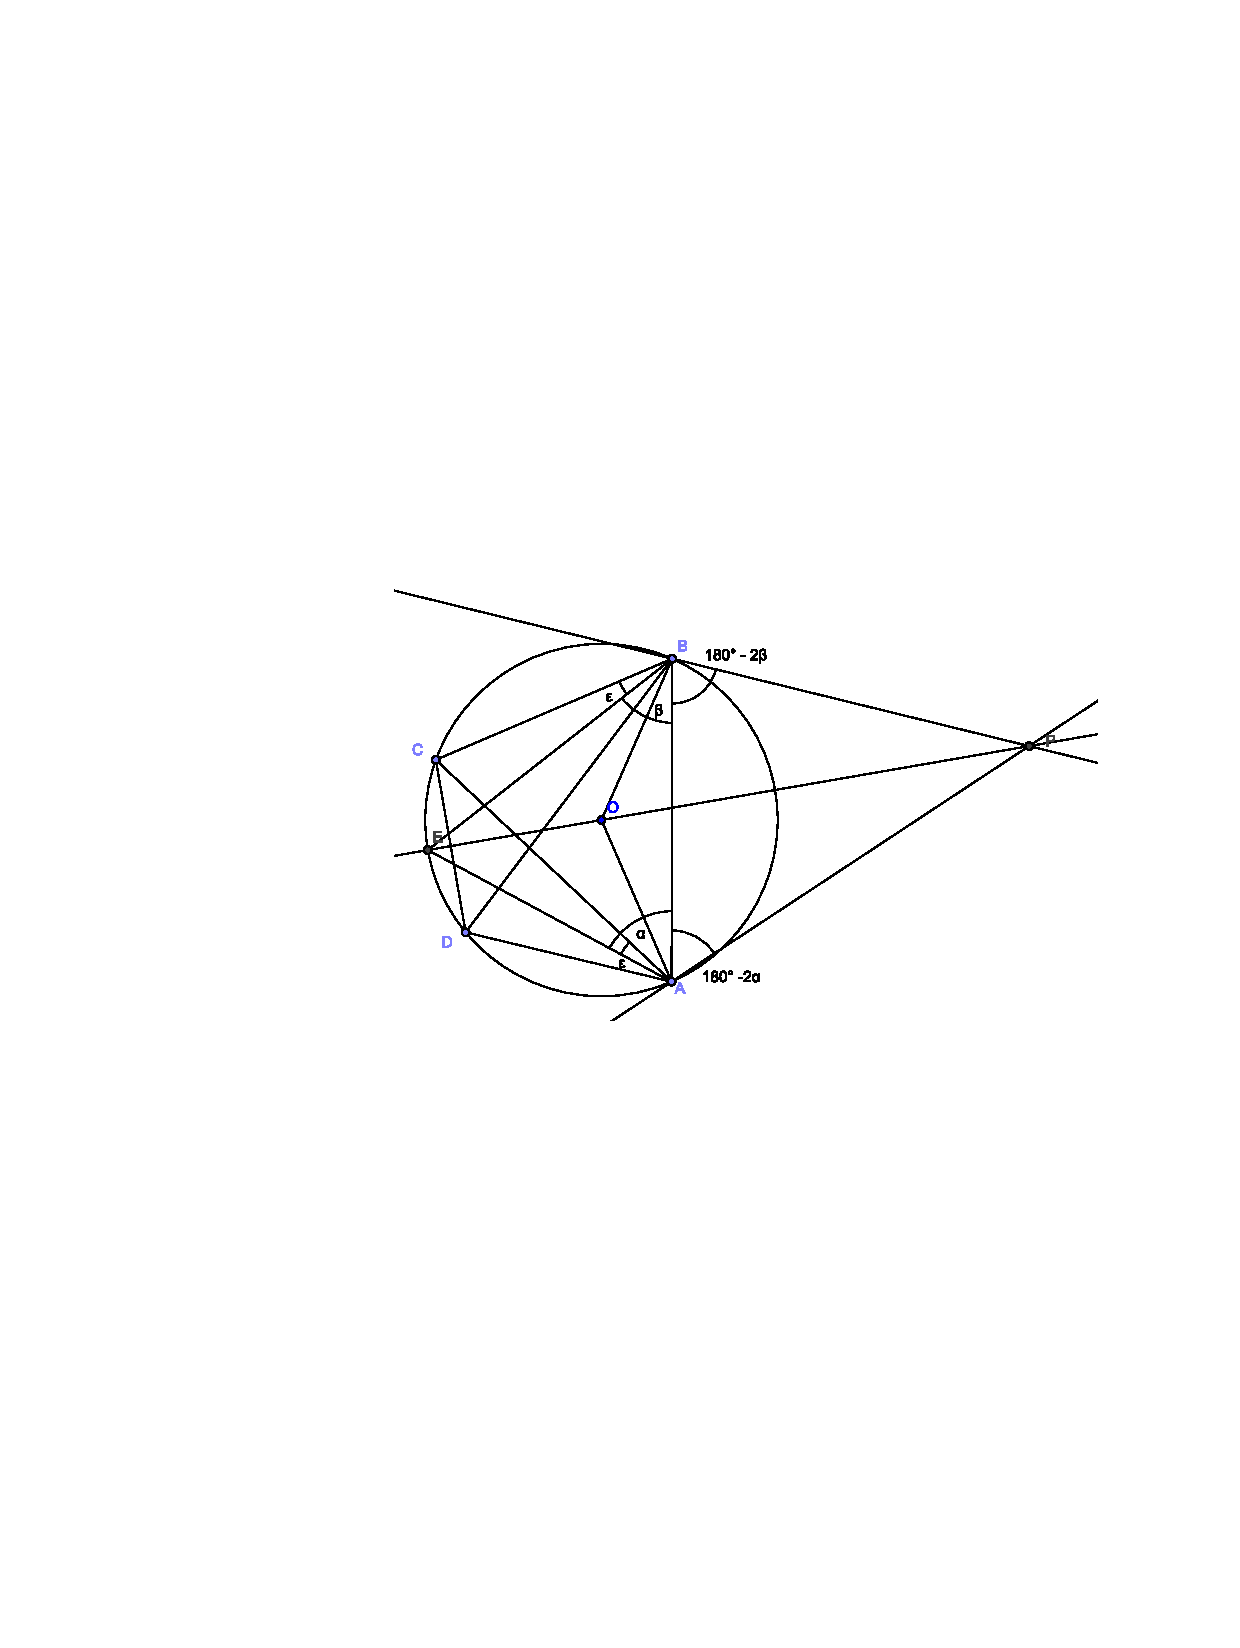
\includegraphics[width=14cm]{aufgabe5b.pdf}
\caption{Aufgabe 5 - Skizze zur zweiten Lösung}
\end{center}
\end{figure}


\emph{Zum Punkteschema:} 
\begin{itemize}
\item $E$ liegt auf dem Kreis 1 Punkt
\item (zusätzlich zum vorigen Punkt) $E$ liegt auf der Mittelsenkrechten +1 Punkt
 \item $PBOA$ ist ein Sehenviereck 2 Punkte.
 \end{itemize}
          



\end{enumerate}


\end{document}
